
On s'intéresse à la fonction $f$ définie sur $[-5;5]$.

\begin{center}
	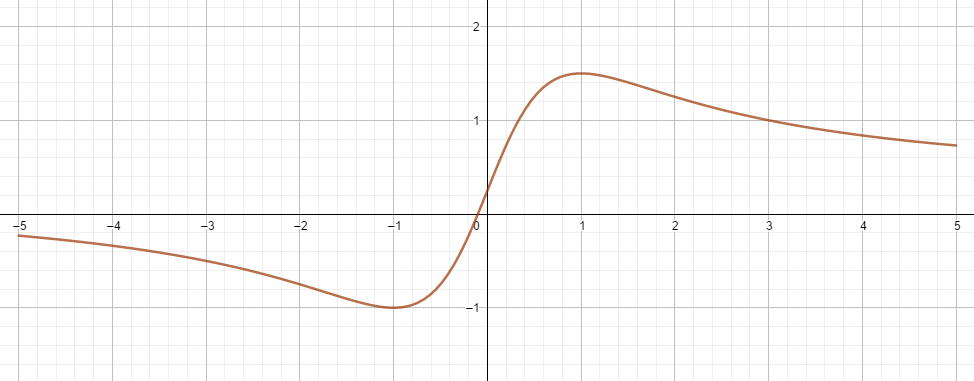
\includegraphics[scale=0.5]{fct}
\end{center}

\begin{questions}
	
	\question[3] Lire graphiquement $f(-3)$, $f(-2)$, $f(-\frac{1}{2})$, $f(0)$, $f(1)$, $f(4)$.
	
	\fillwithdottedlines{2cm}
	
	\question[2] Résoudre les équations suivantes : $f(x)=-1$, $f(x)=0$, $f(x)=1$, $f(x)=2$.
	
	\fillwithdottedlines{3cm}
	
	\question[3] \'Etudier le signe de $f(x)$ sur $[-5;5]$.
	
	\fillwithdottedlines{3cm}
	
	\question[3] \'Etudier les variations de $f(x)$ sur $[-5;5]$.
	
	\fillwithdottedlines{4cm}
\end{questions}